%%%%%%%%%%%%%%%%%%%%%%%%%%%%%%%%%%%%%%%%%%%%%%%%%%%%%%
% A Beamer template for University of Wollongong     %
% Based on THU beamer theme                          %
% Author: Qiuyu Lu                                   %
% Date: July 2024                                    %
% LPPL Licensed.                                     %
%%%%%%%%%%%%%%%%%%%%%%%%%%%%%%%%%%%%%%%%%%%%%%%%%%%%%%
% Customized for Sharif University of Technology     %
%%%%%%%%%%%%%%%%%%%%%%%%%%%%%%%%%%%%%%%%%%%%%%%%%%%%%%


\documentclass[serif, aspectratio=169]{beamer}
%\documentclass[serif]{beamer}  % for 4:3 ratio
\usepackage[T1]{fontenc} 
\usepackage{fourier} % see "http://faq.ktug.org/wiki/uploads/MathFonts.pdf" for other options
\usepackage{hyperref}
\usepackage{latexsym,amsmath,xcolor,multicol,booktabs,calligra}
\usepackage{graphicx,pstricks,listings,stackengine}
\usepackage{lipsum}

% For writing clean pseudocodes
\usepackage{algorithm, algpseudocode, mathtools, needspace}
% To justify the items
\usepackage{ragged2e}
% To draw diagrams
\usepackage{tikz}
% To include urls
\usepackage{url}
% To make clean tables
\usepackage{color, tabularray}

\author{Ali Sharifi-Zarchi}
\title{Machine Learning (CE 40717)}
\subtitle{Fall 2025}
\institute{
    CE Department \\
    Sharif University of Technology
}
\usepackage{SUTstyle}

% defs
\def\cmd#1{\texttt{\color{red}\footnotesize $\backslash$#1}}
\def\env#1{\texttt{\color{blue}\footnotesize #1}}
\definecolor{deepblue}{rgb}{0,0,0.5}
\definecolor{deepred}{RGB}{153,0,0}
\definecolor{deepgreen}{rgb}{0,0.5,0}
\definecolor{halfgray}{gray}{0.55}
\definecolor{silver}{rgb}{0.752,0.752,0.752}

\lstset{
    basicstyle=\ttfamily\small,
    keywordstyle=\bfseries\color{deepblue},
    emphstyle=\ttfamily\color{deepred},    % Custom highlighting style
    stringstyle=\color{deepgreen},
    numbers=left,
    numberstyle=\small\color{halfgray},
    rulesepcolor=\color{red!20!green!20!blue!20},
    frame=shadowbox,
}

% For writing comments that are aligned to the left side
\makeatletter
\NewDocumentCommand{\LeftComment}{s m}{%
  \Statex \IfBooleanF{#1}{\hspace*{\ALG@thistlm}}\(\triangleright\) #2}
\makeatother
% To manually indent states in algorithmicx
\newcommand{\IndState}{\State\hspace{\algorithmicindent}}
% To make breakable algorithms
\makeatletter
\newenvironment{nofloatalgorithmic}[2][0]
  {
  \par
  \needspace{\dimexpr\baselineskip+6.8pt}
  \noindent
  \hrule height.8pt depth0pt \kern2pt
  \refstepcounter{algorithm}
  \addcontentsline{loa}{algorithm}{\numberline{\thealgorithm}#2}
  \noindent\textbf{\fname@algorithm~\thealgorithm} #2\par
  \kern2pt\hrule\kern2pt
  \begin{algorithmic}[#1]
  }
  {
  \end{algorithmic}
  \nobreak\kern2pt\hrule\relax
  }
\makeatother
% To make vertical arrow
\newcommand\vertarrowbox[3][6ex]{%
  \begin{array}[t]{@{}c@{}} #2 \\
  \left\uparrow\vcenter{\hrule height #1}\right.\kern-\nulldelimiterspace\\
  \makebox[0pt]{\scriptsize#3}
  \end{array}%
}
% Clean argmin
\DeclareMathOperator*{\argmin}{arg\,min}

\begin{document}

\begin{frame}
    \titlepage
    \vspace*{-0.6cm}
    \begin{figure}[htpb]
        \begin{center}
            \includegraphics[keepaspectratio, scale=0.25]{pic/sharif-main-logo.png}
        \end{center}
    \end{figure}
\end{frame}

\begin{frame}    
\tableofcontents[sectionstyle=show,
subsectionstyle=show/shaded/hide,
subsubsectionstyle=show/shaded/hide]
\end{frame}

\section{Introduction and Motivation}
%------------------------------------slide1
\begin{frame}{Support Vector Machines (SVMs)}

\begin{itemize}
    \item Developed in the 1990’s by Vapnik and colleagues at Bell Labs based on statistical learning theory
    \item One of the most popular learning techniques until deep learning resurgence
    \item What is interesting about SVMs
    \begin{itemize}
        \item \textbf{Generalization properties}, including achieving a margin and structural risk minimization
        \item Extension to non-linear classifier via \textbf{kernels}
        \item Dual form that shows how \textbf{linear classifiers can be seen as a weighted average of training examples}
        \item Optimization via \textbf{stochastic gradient descent}, also used for neural networks
    \end{itemize}
\end{itemize}

\end{frame}
%------------------------------------slide2
\begin{frame}{What is the best linear classifier?}

\begin{columns}[T] ر
    \begin{column}{0.6\textwidth}
        \begin{itemize}
            \item \textbf{Logistic regression}
            \begin{itemize}
                \item Maximize expected likelihood of label given data
                \item Every example contributes to loss
            \end{itemize}
            
            \vspace{0.5em}
            \item \textbf{SVM}
            \begin{itemize}
                \item Make all examples at least minimally confident
                \item Base decision on a minimal set of examples
            \end{itemize}
        \end{itemize}
    \end{column}

    \begin{column}{0.4\textwidth}
        \centering
        \includegraphics[width=\linewidth]{pic/motiv1.png}
    \end{column}
\end{columns}

\end{frame}
%-----------------------------------slide3
\begin{frame}{Multiple optimal solutions?}

\begin{columns}[T] ر
    \begin{column}{0.5\textwidth}
\begin{itemize}
    \item Given training data $\{(x_i, y_i) : 1 \le i \le n\}$ i.i.d. from distribution $D$
    
    \item Hypothesis 
    \[
        y = \text{sign}(f_w(x)) = \text{sign}(w^T x)
    \]
    \begin{itemize}
        \item {$y = +1$} if {$w^T x > 0$}
        \item {$y = -1$} if {$w^T x < 0$}
    \end{itemize}
    
    \vspace{0.5em}
    \item Let’s assume that we can optimize to find {$w$}
\end{itemize}
    \end{column}

    \begin{column}{0.5\textwidth}
        \centering
        \includegraphics[scale=0.3]{pic/princeton1.jpg}\\
Same on empirical loss\\
Different on test/expected loss
    \end{column}
\end{columns}

\end{frame}
%-----------------------------------slide4

\begin{frame}{What is better linear separation?}
Which Separator Do You Pick?
    \begin{figure}
        \centering
        \includegraphics[scale=0.4]{pic/princeton1.jpg}
    \end{figure}
\end{frame}
%-----------------------------------slide5
\begin{frame}{What is better linear separation?}
    \begin{figure}
        \centering
        \includegraphics[scale=0.4]{pic/princeton2.jpg}
    \end{figure}
\end{frame}
%-----------------------------------slide6
\begin{frame}{What is better linear separation?}
    \begin{figure}
        \centering
        \includegraphics[scale=0.4]{pic/princeton3.jpg}
    \end{figure}
\end{frame}
%-----------------------------------slide7
\begin{frame}{What is better linear separation?}
    \begin{figure}
        \centering
        \includegraphics[scale=0.4]{pic/princeton4.jpg}
    \end{figure}
\end{frame}
%-----------------------------------slide8
\begin{frame}{What is better linear separation?}
Larger margin provides better generalization to unseen data.
    \begin{figure}
        \centering
        \includegraphics[scale=0.4]{pic/princeton5.jpg}
    \end{figure}
\end{frame}
%-----------------------------------slide9
\begin{frame}{SVM Terminology}

\begin{columns}[T]

    \begin{column}{0.6\textwidth}
        \includegraphics[width=\linewidth]{pic/terminology.png}

    \end{column}

    \begin{column}{0.4\textwidth}
        \textbf{\textcolor{blue}{Support Vector}}: training observations whose distance to the hyperplane is equal to the margin

        \vspace{1em}

        \textbf{\textcolor{orange}{Margin}}:smallest distance between any training observation and the hyperplane.

    \end{column}
\end{columns}

\end{frame}

%-----------------------------------slide
\begin{frame}{Fat Hyperplane}
We call such hyperplanes fat
   \begin{figure}
        \centering
        \includegraphics[scale=0.2]{pic/SVM2.png}
    \end{figure}
    \begin{figure}
        \centering
        \includegraphics[scale=0.2]{pic/SVM3.png}
    \end{figure}
\end{frame}
%-----------------------------------slide10
\begin{frame}{SVMs minimize $\mathbf{w^T w}$ while preserving a margin of 1}

\begin{columns}[T]
    \begin{column}{0.5\textwidth}
        \centering
        Optimized SVM \\[0.5em]
        \includegraphics[width=\linewidth]{pic/logistic1.png}
      
        \vspace{0.5em}
        \footnotesize Decision boundary depends only on\\
        “support vectors” (circled)
    \end{column}

    \begin{column}{0.5\textwidth}
        \centering
        Optimized Linear Logistic Regression\\[0.5em]
        \includegraphics[width=\linewidth]{pic/logistic2.png}
        
        \vspace{0.5em}
        \footnotesize Minimizes the sum of logistic error on all samples,\\
        so boundary should be further from dense regions
    \end{column}
\end{columns}

\end{frame}

\section{Hard-Margin SVM}
%-----------------------------------slide11
\begin{frame}{Why is it called a support vector?}

\begin{itemize}
    \item \textbf{Support}: maximal margin hyperplane only depends on these observations.
    \vspace{1em}
    \item \textbf{Vector}: points are vectors in $p$-dimensional space.
\end{itemize}

\vspace{1em}

If support vectors are perturbed, then MM hyperplane will change.

\vspace{1em}

If other training observations perturbed (provided not perturbed within margin distance of hyperplane), then MM hyperplane not affected.

\end{frame}

%-----------------------------------slide11
\begin{frame}{Finding {\textbf{w}} with large margin}

Let ${x_n}$ be the nearest data point to the plane 
\[
    {w}^\top {x} = 0.
\]
How far is it? 2 preliminary technicalities:

\raggedright
1. Normalize $w$:
\[
    \left| {w}^\top {x_n} \right| = 1
\]


2. Pull out $w_0$:

\[
    {w} = (w_1, \cdots, w_d)
\]
apart from $b$.


The plane is now 
\[
    {w}^\top {x} + b = 0
\]

\end{frame}

%-----------------------------------slide11
\begin{frame}{Computing the distance}

The distance between $\mathbf{x}_n$ and the plane {$\mathbf{w}^{\top}\mathbf{x} + b = 0$} 
\quad where \quad $|{\mathbf{w}^{\top}\mathbf{x}_n + b}| = 1$

\vspace{1em}

The vector {$\mathbf{w}$} is $\perp$ to the plane in the $\mathcal{X}$ space:

\vspace{1em}

Take $\mathbf{x}'$ and $\mathbf{x}''$ on the plane

\[
{\mathbf{w}^{\top}\mathbf{x}'} + b = 0 
\quad \text{and} \quad 
{\mathbf{w}^{\top}\mathbf{x}''} + b = 0
\Longrightarrow \quad {\mathbf{w}^{\top}} (\mathbf{x}' - \mathbf{x}'') = 0
\]


\begin{center}
\includegraphics[width=0.5\linewidth]{pic/A1.png}
\end{center}

\end{frame}
%----------------------------------------slide
\begin{frame}{and the distance is \dots}

Distance between $\mathbf{x}_n$ and the plane: Take any point $\mathbf{x}$ on the plane Projection of $\mathbf{x}_n - \mathbf{x}$ on {$\mathbf{w}$}

\[
\hat{\mathbf{w}} = \frac{{\mathbf{w}}}{\|{\mathbf{w}}\|} 
\quad \Longrightarrow \quad
\text{distance} = \big| \hat{\mathbf{w}}^{\top} (\mathbf{x}_n - \mathbf{x}) \big|
\]

\[
\text{distance} = \frac{1}{\|{\mathbf{w}}\|} 
\big|{\mathbf{w}^{\top}\mathbf{x}_n - \mathbf{w}^{\top}\mathbf{x}} \big|
= \frac{1}{\|{\mathbf{w}}\|} 
\big| {\mathbf{w}^{\top}\mathbf{x}_n + b - \mathbf{w}^{\top}\mathbf{x} - b} \big|
= \frac{1}{\|{\mathbf{w}}\|}
\]


\begin{center}
\includegraphics[width=0.5\linewidth]{pic/A2.png}
\end{center}

\end{frame}

%-----------------------------------------slide
\begin{frame}{The optimization problem}

Maximize $\frac{1}{\|\mathbf{w}\|} $ \\
subject to $ \min_{n=1,2,\ldots,N} |\mathbf{w}^{\top}\mathbf{x}_n + b| = 1 $\\

\vspace{1em}
Notice: $ |\mathbf{w}^{\top}\mathbf{x}_n + b| = y_n (\mathbf{w}^{\top}\mathbf{x}_n + b) $ \\

\vspace{1em}
Minimize $ \frac{1}{2}\mathbf{w}^{\top}\mathbf{w} $ \\
subject to $
y_n(\mathbf{w}^{\top}\mathbf{x}_n + b) \ge 1 
\quad \text{for} \quad n = 1,2,\ldots,N $ 
\[
\mathbf{w} \in \mathbb{R}^d, \quad b \in \mathbb{R}
\]
\vspace{1em}
Lagrange? \quad inequality constraints $\Longrightarrow$ KKT

\end{frame}
%----------------------------------------slide
\begin{frame}{Lagrange formulation}

Minimize $
\mathcal{L}(\mathbf{w}, b, \boldsymbol{\alpha}) 
= \frac{1}{2} \mathbf{w}^{\top}\mathbf{w}
- \sum_{n=1}^{N} \alpha_n \big( y_n(\mathbf{w}^{\top}\mathbf{x}_n + b) - 1 \big) $

\vspace{2em}

w.r.t. $\mathbf{w}$ and $b$ and maximize w.r.t. each $\alpha_n \ge 0$

\[
\nabla_{\mathbf{w}}\mathcal{L} 
= \mathbf{w} - \sum_{n=1}^{N} \alpha_n y_n \mathbf{x}_n = 0
\]

\[
\frac{\partial \mathcal{L}}{\partial b} 
= - \sum_{n=1}^{N} \alpha_n y_n = 0
\]

\end{frame}
%-----------------------------------------slide
\begin{frame}{Substituting}

\[
\mathbf{w} = \sum_{n=1}^{N} \alpha_n y_n \mathbf{x}_n 
\quad \text{and} \quad 
\sum_{n=1}^{N} \alpha_n y_n = 0
\]

\vspace{2em}
in the Lagrangian
$
\quad \mathcal{L}(\mathbf{w}, b, \boldsymbol{\alpha}) 
= \frac{1}{2} \mathbf{w}^{\top}\mathbf{w} 
- \sum_{n=1}^{N} \alpha_n \big( y_n(\mathbf{w}^{\top}\mathbf{x}_n + b) - 1 \big)
$\\
\vspace{2em}
we get $
\quad \mathcal{L}(\boldsymbol{\alpha}) 
= \sum_{n=1}^{N} \alpha_n 
- \frac{1}{2} \sum_{n=1}^{N} \sum_{m=1}^{N} 
y_n y_m \alpha_n \alpha_m \mathbf{x}_n^{\top}\mathbf{x}_m
$\\
\vspace{2em}
Maximize w.r.t. $\boldsymbol{\alpha}$ subject to $
\quad \alpha_n \ge 0 \quad \text{for } n = 1, \dots, N 
\quad \text{and} \quad 
\sum_{n=1}^{N} \alpha_n y_n = 0
$\\

\end{frame}

%-----------------------------------------slide
\begin{frame}{The solution – quadratic programming}

\[
\min_{\boldsymbol{\alpha}} 
\frac{1}{2} \boldsymbol{\alpha}^\top
\begin{bmatrix}
y_1 y_1 \mathbf{x}_1^\top \mathbf{x}_1 & y_1 y_2 \mathbf{x}_1^\top \mathbf{x}_2 & \dots & y_1 y_N \mathbf{x}_1^\top \mathbf{x}_N \\
y_2 y_1 \mathbf{x}_2^\top \mathbf{x}_1 & y_2 y_2 \mathbf{x}_2^\top \mathbf{x}_2 & \dots & y_2 y_N \mathbf{x}_2^\top \mathbf{x}_N \\
\vdots & \vdots & \ddots & \vdots \\
y_N y_1 \mathbf{x}_N^\top \mathbf{x}_1 & y_N y_2 \mathbf{x}_N^\top \mathbf{x}_2 & \dots & y_N y_N \mathbf{x}_N^\top \mathbf{x}_N
\end{bmatrix}
\boldsymbol{\alpha}
+ (-\mathbf{1}^\top)\boldsymbol{\alpha}
\]

subject to
\[
\mathbf{y}^\top \boldsymbol{\alpha} = 0
\quad \text{and} \quad
\mathbf{0} \le \boldsymbol{\alpha} \le \infty
\]

\end{frame}
%-----------------------------------------slide
\begin{frame}{Non-Separable Data}
    \begin{columns}
        \column{0.5\textwidth}
        \centering
        \includegraphics[width=0.7\linewidth]{pic/SVM6.jpg} \\
        Tolerate error

        \column{0.5\textwidth}
        \centering
        \includegraphics[width=0.7\linewidth]{pic/SVM7.jpg} \\
        Nonlinear transform
    \end{columns}
\end{frame}

%-----------------------------------------slide
\begin{frame}{Introduce slack variables}

\begin{columns}
    \begin{column}{0.4\textwidth}
        Margin violation: \quad $y_n (w^{\top} x_n + b) \ge 1$ fails
        
        \vspace{1em}
        Quantify: \quad $y_n (w^{\top} x_n + b) \ge 1\textcolor{red}{ - \xi_n}$, \quad $\textcolor{red}{\xi_n }\ge 0$
        
        \vspace{1em}
        Total violation \quad $= \sum_{n=1}^{N} \textcolor{red}{\xi_n}$

\begin{itemize}
    \item for $0 < \xi \le 1$ point is between margin and correct side of hyperplane. 
    This is a \textbf{margin violation}
    \vspace{0.5em}
    \item for $\xi > 1$ point is \textbf{misclassified}
\end{itemize}
    \end{column}
    \begin{column}{0.6\textwidth}
        \centering
        \includegraphics[width=\linewidth]{pic/slack.png}
    \end{column}
\end{columns}

\end{frame}
%-----------------------------------------slide

%-----------------------------------------slide
\section{Soft-Margin SVM}

\begin{frame}
\begin{columns}[T]

    \begin{column}{0.5\textwidth}
        \centering
        \includegraphics[width=\linewidth]{pic/nonlin1.png}

    \end{column}


    \begin{column}{0.5\textwidth}
        \centering
        \includegraphics[width=0.9\linewidth]{pic/nonlin2.png}

    \end{column}
\end{columns} 
\end{frame}

%-----------------------------------------slide
\begin{frame}{Soft Margin SVM}

\begin{columns}[T]
    \begin{column}{0.6\textwidth}
        \begin{align*}
            &\text{minimize}_{b, {w}, {\xi}} \quad 
            \frac{1}{2}{w}^\top {w} 
            \textcolor{red}{+ {C \sum_{n=1}^{N} \xi_n}} \\
            &\text{subject to:} \quad 
            y_n({w}^\top {x_n} + b) \ge 1 \textcolor{red}{- \xi_n} \quad \text{for } n = 1, \ldots, N\\
            & \hspace{6em} \xi_n \ge 0 \quad \text{for } n = 1, \ldots, N \\
           &\hspace{6em} w \in \mathbb{R}^{d}, \quad b \in \mathbb{R}, \quad  \textcolor{red}{\xi \in \mathbb{R}^{N}}
        \end{align*}
    \end{column}

    \begin{column}{0.4\textwidth}
        \centering
        \includegraphics[width=0.9\linewidth]{pic/soft.png}
    \end{column}

\end{columns}

\end{frame}
%-----------------------------------------slide
\begin{frame}{Soft Margin SVM}
\begin{itemize}
\item   Trades off ‘soft in-sample error’ 
        $\displaystyle \sum_{n=1}^{N}\xi_n$ 
        with weight norm 
        $\displaystyle \frac{1}{2} {w}^\top {w}$
    \item Every constraint can be satisfied if $\xi_i$ is sufficiently large
    \vspace{0.5em}
    \item $C$ is a \textbf{regularization} parameter:
    \begin{itemize}
        \item small $C$ allows constraints to be easily ignored $\rightarrow$ large margin
        \item large $C$ makes constraints hard to ignore $\rightarrow$ narrow margin
        \item $C = \infty$ enforces all constraints: hard margin
    \end{itemize}
    \vspace{0.5em}
    \item This is still a quadratic optimization problem and there is a unique minimum. 
    Note, there is only one parameter, $C$.
\end{itemize}
\end{frame}
%-----------------------------------------slide

\begin{frame}{Non-Separable Data}

\begin{columns}[T]

    \begin{column}{0.5\textwidth}
        \centering
        \includegraphics[width=0.5\linewidth]{pic/soft2.png}

        
        \vspace{0.3em}
        $C = 1$
    \end{column}


    \begin{column}{0.5\textwidth}
        \centering
        \includegraphics[width=0.5\linewidth]{pic/soft3.png}

        
        \vspace{0.3em}
        $C = 500$
    \end{column}
\end{columns} 

\begin{align*}
    &\text{minimize}_{b, w, \xi} \quad 
    \frac{1}{2} w^{\top} w  \textcolor{red}{ +  C \sum_{n=1}^{N} \xi_n}  \\
    &\text{subject to:} \quad 
    y_n(w^{\top} x_n + b) \ge 1  \textcolor{red}{-  \xi_n }  \quad \text{for } n = 1, \ldots, N \\
    &  \hspace{6em} \xi_n \ge 0 \quad \text{for } n = 1, \ldots, N
\end{align*}

\end{frame}

%-----------------------------------------slide
\begin{frame}{Soft Margin SVM With Separable Data}

\begin{columns}[T]
    \begin{column}{0.25\textwidth}
        \centering
        \includegraphics[width=\linewidth]{pic/softmargin1.png}
        \vspace{0.3em}
        small $C$
    \end{column}
    \begin{column}{0.25\textwidth}
        \centering
        \includegraphics[width=\linewidth]{pic/softmargin2.png}
        \vspace{0.3em}
        medium $C$
    \end{column}
    \begin{column}{0.25\textwidth}
        \centering
        \includegraphics[width=\linewidth]{pic/softmargin3.png}
        \vspace{0.3em}
        large $C$
    \end{column}
    \begin{column}{0.25\textwidth}
        \centering
        \includegraphics[width=\linewidth]{pic/softmargin4.png}
        \vspace{0.3em}
        hard margin
    \end{column}
\end{columns}

\begin{columns}[T]
    \begin{column}{0.7\textwidth}
        \centering
\begin{align*}
    &\text{minimize}_{b, w, \xi} \quad 
    \frac{1}{2} w^{\top} w \textcolor{red}{+ C \sum_{n=1}^{N} \xi_n }\\
    &\text{subject to:} \quad 
    y_n(w^{\top} x_n + b) \ge 1 \textcolor{red}{- \xi_n}  \quad \text{for } n = 1, \ldots, N  \\
    & \hspace{6em} \xi_n \ge 0 \quad \text{for } n = 1, \ldots, N
\end{align*}
    \end{column}
    \begin{column}{0.3\textwidth}
        \centering
       \vspace{3em}
       \textbf{Choice of $C$ is IMPORTANT}

    \end{column}
\end{columns}

\end{frame}


%-----------------------------------------slide
\begin{frame}{Lagrange formulation}

\[
\mathcal{L}(w, b, \textcolor{red}{\xi}, {\alpha}, \textcolor{purple}{\beta})
= \frac{1}{2} w^{\top} w 
+ C \sum_{n=1}^{N} \textcolor{red}{\xi_n}
- \sum_{n=1}^{N} {\alpha_n} \big( y_n (w^{\top} x_n + b) - 1 + \textcolor{red}{\xi_n} \big)
- \sum_{n=1}^{N} \textcolor{purple}{\beta_n} \textcolor{red}{\xi_n}
\]

Minimize w.r.t. \textbf{w}, \textbf{b}, and \textcolor{red}{$\xi$} and maximize w.r.t. each {$\alpha_n \ge 0$} and \textcolor{purple}{$\beta_n \ge 0$}

\vspace{1em}

\[
\nabla_w \mathcal{L} = w - \sum_{n=1}^{N} {\alpha_n} y_n x_n = 0
\]

\[
\frac{\partial \mathcal{L}}{\partial b} = - \sum_{n=1}^{N} {\alpha_n} y_n = 0
\]

\[
\frac{\partial \mathcal{L}}{\partial \textcolor{red}{\xi_n}} = C - {\alpha_n} - \textcolor{purple}{\beta_n} = 0
\]

\end{frame}
%------------------------------------------------slide
\begin{frame}{Soft-margin SVM: Dual problem}

\[
\max_{\boldsymbol{\alpha}} 
\left(
\sum_{n=1}^{N} \alpha_n
- \frac{1}{2} 
\sum_{n=1}^{N} \sum_{m=1}^{N}
\alpha_n \alpha_m y_{n} y_{m} 
\mathbf{x}_n^{\top} \mathbf{x}_{m}
\right)
\]

Subject to
\[
\sum_{n=1}^{N} \alpha_n y_{n} = 0,
\quad
0 \le \alpha_n \le C, \quad n = 1, \dots, N
\]

After solving the above quadratic problem, $\mathbf{w}$ is found as:
\[
\mathbf{w} = \sum_{n=1}^{N} \alpha_n y_{n} \mathbf{x}_{n}
\]

\end{frame}
%-----------------------------------------slide
\begin{frame}{Not linearly separable data}

\begin{columns}[T]

\begin{column}{0.55\textwidth}
    \textbf{Noisy data or overlapping classes} \\
    (we discussed about it: soft margin)
    \begin{itemize}
        \item Near linearly separable
    \end{itemize}
\end{column}

\begin{column}{0.45\textwidth}

     \textbf{Non-linear decision surface}
    \begin{itemize}
        \item Transform to a new feature space
    \end{itemize}
\end{column}
\end{columns}

\begin{center}
\includegraphics[width=0.7\textwidth]{pic/transform2.png}
\end{center}

\end{frame}
%-----------------------------------------slide
\begin{frame}{Mechanics of the Nonlinear Transform}

\begin{center}
\includegraphics[width=0.8\textwidth]{pic/transform3.png}
\end{center}

\end{frame}
%-----------------------------------------slide
\begin{frame}{Soft-margin SVM in a transformed space: Primal problem}

\begin{itemize}
    \item \textbf{Primal problem:}
\end{itemize}

\[
\min_{\mathbf{w}, w_0} 
\frac{1}{2}\|\mathbf{w}\|^2 + 
C \sum_{n=1}^{N} \xi_n
\]

subject to:
\[
y_{n} \left( \mathbf{w}^T \textcolor{red}{\phi(x_{(n})} + w_0 \right) \ge 1 - \xi_n, 
\quad n = 1, \ldots, N
\]
\[
\xi_n \ge 0
\]

\vspace{1em}
\begin{itemize}
    \item \(\mathbf{w} \in \mathbb{R}^m\): the weights that must be found.
    \item If \(m \gg d\) (very high-dimensional feature space), then there are many more parameters to learn.
\end{itemize}

\end{frame}
%-----------------------------------------slide
\begin{frame}{Soft-margin SVM in a transformed space: Dual problem}

\begin{itemize}
    \item \textbf{Optimization problem:}
\end{itemize}

\[
\max_{\alpha} 
\left\{
\sum_{n=1}^{N} \alpha_n 
- \frac{1}{2}
\sum_{n=1}^{N}\sum_{m=1}^{N} 
\alpha_n \alpha_m y_{n} y_{m} 
\textcolor{red}{\phi(x_{n})^T \phi(x_{m})}
\right\}
\]

Subject to:
\[
\sum_{n=1}^{N} \alpha_n y_{n} = 0
\]
\[
0 \leq \alpha_n \leq C \quad n = 1, \ldots, N
\]

\vspace{1em}
\begin{itemize}
    \item If we have inner products 
    \(\textcolor{magenta}{\phi(x_{i})^T \phi(x_{j})}\),
    only \(\boldsymbol{\alpha = [\alpha_1, \ldots, \alpha_N]}\) 
    needs to be learned.
    \item Not necessary to learn \(m\) parameters as opposed to the primal problem.
\end{itemize}

\end{frame}

%-----------------------------------------slide
\begin{frame}{Classifying a new data}

\[
\hat{y} = sign(w_0 + \mathbf{w}^T \textcolor{red}{\phi(x)})
\]

\[
\text{where } \mathbf{w} = \sum_{\alpha_n > 0} \alpha_n y_{n} \textcolor{red}{\phi(x_{n})}
\]

\[
\text{and } w_0 = y_{s} - \mathbf{w}^T \textcolor{red}{\phi(x_{s})}
\]

\end{frame}
%-----------------------------------------slide
\begin{frame}{Not linearly separable data}

\begin{columns}[T]

\begin{column}{0.5\textwidth}
\begin{center}
\includegraphics[width=0.7\textwidth]{pic/inkernel1.png}
\end{center}
\end{column}

\begin{column}{0.5\textwidth}
\begin{center}
\includegraphics[width=0.7\textwidth]{pic/inkernel2.png}
\end{center}
\end{column}
\end{columns}

\end{frame}
%-----------------------------------------slide
\section{Kernel SVM}

%-----------------------------------------slide
\begin{frame}{Kernel SVM}

\begin{itemize}
    \item Learns linear decision boundary in a high-dimensional space without explicitly working on the mapped data.
    
    \vspace{1em}
    \item Let 
    \[
    {\phi(x)^T \phi(x')} = {K(x, x')}
    \quad \text{(kernel)}
    \]
    
    \vspace{1em}
    \item Example: 
    \[
    x = [x_1, x_2]
    \quad \text{and second-order } {\phi}:
    \]
    \[
    {\phi(x)} = [1, x_1, x_2, x_1^2, x_2^2, x_1x_2]
    \]
\end{itemize}

\vspace{1em}
Then,
\[
{K(x, x')} 
= 1 + x_1x'_1 + x_2x'_2 + x_1^2x_1'^2 + x_2^2x_2'^2 + x_1x'_1x_2x'_2
\]

\end{frame}
%-----------------------------------------slide
\begin{frame}{Kernel trick}

\begin{itemize}
    \item Compute ${K(x, x')}$ without transforming ${x}$ and ${x'}$.
    
    \vspace{1em}
    \item Example: Consider 
    \[
    {K}(x, x') = (1 + x^T x')^2
    \]
    \[
    = (1 + x_1x'_1 + x_2x'_2)^2
    \]
    \[
    = 1 + {2x_1x'_1} + {2x_2x'_2} + x_1^2x_1'^2 + x_2^2x_2'^2 + {2x_1x'_1x_2x'_2}
    \]
\end{itemize}

\vspace{1em}
This is an inner product in:

\[
{\phi}(x) = [1, \sqrt{2}x_1, \sqrt{2}x_2, x_1^2, x_2^2, \sqrt{2}x_1x_2]
\]

\[
{\phi}(x') = [1, \sqrt{2}x'_1, \sqrt{2}x'_2, x_1'^2, x_2'^2, \sqrt{2}x'_1x'_2]
\]

\end{frame}

%-----------------------------------------slide
\begin{frame}{Polynomial kernel: Degree two}

\begin{itemize}
    \item We instead use 
    \[
    {K}(x, x') = (x^T x' + 1)^2
    \]
    that corresponds to:
    
    \vspace{0.5em}
    {$d$-dimensional feature space:} 
    \[
    x = [x_1, \ldots, x_d]^T
    \]
    
    \vspace{0.5em}
    \[
    \phi(x) = 
    [1, \sqrt{2}x_1, \ldots, \sqrt{2}x_d, x_1^2, \ldots, x_d^2, 
    \sqrt{2}x_1x_2, \ldots, \sqrt{2}x_1x_d, 
    \sqrt{2}x_2x_3, \ldots, \sqrt{2}x_{d-1}x_d]^T
    \]
\end{itemize}

\end{frame}
%-----------------------------------------slide
\begin{frame}{Polynomial kernel}

\begin{itemize}
    \item This can similarly be generalized to $d$-dimensional $x$ and $\phi$s are polynomials of order $M$:
    \[
    {K}(x, x') = (1 + x^T x')^{M}
    \]
    \[
    = (1 + x_1 x'_1 + x_2 x'_2 + \cdots + x_d x'_d)^{M}
    \]
    
    \vspace{1em}
    \item Example: SVM boundary for a polynomial kernel
    \[
    w_0 + w^T \phi(x) = 0
    \]
    \[
    \Rightarrow w_0 + \sum_{\alpha_i > 0} \alpha_i y_{i} \phi(x_{i})^T \phi(x) = 0
    \]
    \[
    \Rightarrow w_0 + \sum_{\alpha_i > 0} \alpha_i y_{i} k(x_{i}, x) = 0
    \]\\
    
    $\Rightarrow w_0 + \sum_{\alpha_i > 0} \alpha_i y_{i} (1 + x_i^{T}x)^{M} = 0 \quad \rightarrow \quad $ Boundary is a polynomial of order M
\end{itemize}

\end{frame}
%-----------------------------------------slide
\begin{frame}{Why kernel?}

\begin{itemize}
    \item Kernel functions ${K}$ can indeed be efficiently computed, with a cost proportional to ${d}$ (the dimensionality of the input) instead of ${m}$.

    \vspace{1em}
    \item \textbf{Example:} consider the second-order polynomial transform:
    \[
    {\phi}(x) = [1, x_1, \ldots, x_d, x_1^2, x_1x_2, \ldots, x_d x_d]^T 
    \quad {m = 1 + d + d^2}
    \]
    
    \[
    {\phi}(x)^T {\phi}(x') 
    = 1 + \sum_{i=1}^{d} x_i x'_i 
    + \sum_{i=1}^{d} \sum_{j=1}^{d} x_i x_j x'_i x'_j 
    \quad {O(m)}
    \]
    
    \[
    {\phi}(x)^T {\phi}(x') 
    = 1 + (x^T x') + (x^T x')^2 
    \quad {O(d)}
    \]
\end{itemize}

\end{frame}
%-----------------------------------------slide
\begin{frame}{Nonlinear Transform and SVM}

\begin{columns}[T]

\begin{column}{\textwidth}
\centering
\includegraphics[width=0.9\textwidth]{pic/whykernel.png}
\end{column}

\end{columns}

\begin{itemize}
    \item $\Phi_3$ has almost $2\times$ the parameters of $\Phi_2$
    \item $\Phi_3$-SVM does not display significant overfitting compared to $\Phi_3$-regression
    \item support vectors did not double
    \item Can go to higher dimensions if support vectors stays small or margin stays large
\end{itemize}

\end{frame}

%-----------------------------------------slide
\begin{frame}{Gaussian or RBF kernel}

\begin{itemize}
    \item If ${K}(x, x')$ is an inner product in some transformed space of $x$, it is good.
    
    \vspace{0.7em}
    \item ${K}(x, x') = \exp\left(-\frac{\|x - x'\|^2}{\gamma}\right)$
    
    \vspace{0.7em}
    \item Take one dimensional case with $\gamma = 1$:
    \[
    {K}(x, x') = \exp\left(-(x - x')^2\right)
    \]
    \[
    = \exp(-x^2)\exp(-x'^2)\exp(2xx')
    \]
    \[
    = \textcolor{red}{\exp(-x^2)} \,
      \textcolor{magenta}{\exp(-x'^2)} 
      \sum_{k=1}^{\infty} 
      \frac{\textcolor{green!50!black}{2^k} x^k x'^k}{\textcolor{green!50!black}{k!}}	
    \]
\end{itemize}

\end{frame}

%-----------------------------------------slide
\begin{frame}{Some common kernel functions}

\begin{itemize}
    \item \textbf{Linear:} \quad 
    $k(x, x') = x^{T}x'$
    
    \vspace{0.5em}
    \item \textbf{Polynomial:} \quad 
    $k(x, x') = (x^{T}x' + 1)^{M}$
    
    \vspace{0.5em}
    \item \textbf{Gaussian:} \quad 
    $k(x, x') = 
    \exp\left(-\frac{\|x - x'\|^{2}}{\gamma}\right)$
    
    \vspace{0.5em}
    \item \textbf{Sigmoid:} \quad 
    $k(x, x') = 
    \tanh(a\,x^{T}x' + b)$
\end{itemize}

\end{frame}


%-----------------------------------------slide
\begin{frame}{Kernel formulation of SVM}

Optimization problem:

\[
\max_{\boldsymbol{\alpha}} 
\left\{
\sum_{n=1}^{N} \alpha_n 
- \frac{1}{2} 
\sum_{n=1}^{N}\sum_{m=1}^{N} 
\alpha_n \alpha_m y_{n} y_{m} 
\textcolor{red}{k(\mathbf{x}_{n}, \mathbf{x}_{m})}
\right\}
\]

\[
\text{Subject to } 
\sum_{n=1}^{N} \alpha_n y_{n} = 0
\]
\[
0 \leq \alpha_n \leq C \quad n = 1, \ldots, N
\]

\[
\mathbf{Q} =
\begin{bmatrix}
y_{1}y_{1}K(\mathbf{x}_{1}, \mathbf{x}_{1}) & \cdots & y_{1}y_{N}K(\mathbf{x}_{1}, \mathbf{x}_{N}) \\
\vdots & \ddots & \vdots \\
y_{N}y_{1}K(\mathbf{x}_{N}, \mathbf{x}_{1}) & \cdots & y_{N}y_{N}K(\mathbf{x}_{N}, \mathbf{x}_{N})
\end{bmatrix}
\]

\end{frame}

%-----------------------------------------slide
\begin{frame}{Gaussian kernel}

     \textbf{Example:} SVM boundary for a Gaussian kernel
    \begin{itemize}
        \item Considers a Gaussian function around each data point.
        \[
        w_0 + \sum_{\alpha_i > 0} \alpha_i y^{(i)} 
        \exp\left(-\frac{\|\mathbf{x} - \mathbf{x}^{(i)}\|^2}{\sigma}\right) = 0
        \]
        \item SVM + Gaussian Kernel can classify any arbitrary training set
        \begin{itemize}
            \item Training error is zero when $\sigma \to 0$
            \begin{itemize}
                \item All samples become support vectors (likely overfitting)
            \end{itemize}
        \end{itemize}
    \end{itemize}

\end{frame}

%------------------------------------------------slide
\begin{frame}{Hard margin Example}
\begin{center}
\includegraphics[width=0.9\textwidth]{pic/hardmargin.png}
\end{center}

For narrow Gaussian (large  $\sigma$), even the protection of a large margin cannot suppress overfitting.

\end{frame}

%-----------------------------------------slide

\begin{frame}
\begin{columns}[T]

    \begin{column}{0.5\textwidth}
        \centering
\quad SVM with a polynomial kernel of degree 3
        \includegraphics[width=0.75\linewidth]{pic/nonlin3.png}
\[
{K}(x_i, x_i') = 
\left( 1 + \sum_{j=1}^{p} x_{ij} x'_{ij} \right)^{d}
\]

    \end{column}


    \begin{column}{0.5\textwidth}
        \centering
\quad \quad SVM with a radial kernel
        \includegraphics[width=0.77\linewidth]{pic/nonlin4.png}
\[
{K}(x_i, x_i') = 
\exp\left(-\gamma \sum_{j=1}^{p} (x_{ij} - x'_{ij})^2 \right)
\]


    \end{column}
\end{columns} 
\end{frame}

%-----------------------------------------slide

%------------------------------------------------slide
\begin{frame}{SVM Gaussian kernel: Example}

\[
f(\mathbf{x}) = w_0 + \sum_{\alpha_i > 0} \alpha_i y^{(i)} 
\exp\left(-\frac{\|\mathbf{x} - \mathbf{x}^{(i)}\|^2}{2\sigma^2}\right)
\]

\begin{center}
\includegraphics[width=0.6\textwidth]{pic/kernel.png}
\end{center}

\end{frame}

%------------------------------------------------slide
\begin{frame}{SVM Gaussian kernel: Example}

\begin{center}
\includegraphics[width=0.8\textwidth]{pic/kernel1.png}
\end{center}

\end{frame}

%------------------------------------------------slide

\begin{frame}{SVM Gaussian kernel: Example}

\begin{center}
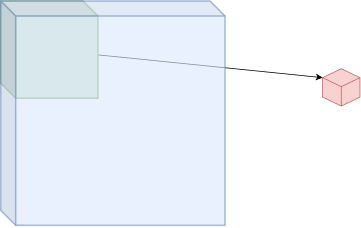
\includegraphics[width=0.7\textwidth]{pic/kernel2.png}
\end{center}

\end{frame}
%------------------------------------------------slide

\begin{frame}{SVM Gaussian kernel: Example}

\begin{center}
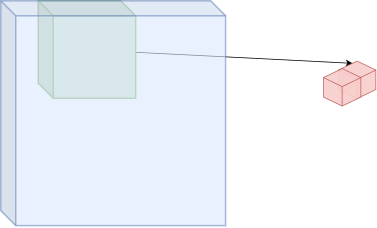
\includegraphics[width=0.7\textwidth]{pic/kernel3.png}
\end{center}

\end{frame}

%------------------------------------------------slide
\begin{frame}{SVM Gaussian kernel: Example}

\begin{center}
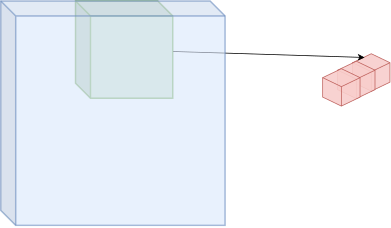
\includegraphics[width=0.7\textwidth]{pic/kernel4.png}
\end{center}

\end{frame}

%------------------------------------------------slide

\begin{frame}{SVM Gaussian kernel: Example}

\begin{center}
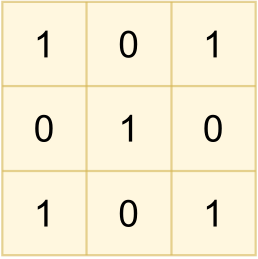
\includegraphics[width=0.7\textwidth]{pic/kernel5.png}
\end{center}

\end{frame}
%------------------------------------------------slide
\begin{frame}{SVM Gaussian kernel: Example}

\begin{center}
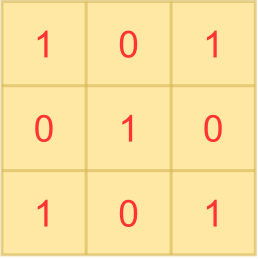
\includegraphics[width=0.7\textwidth]{pic/kernel6.png}
\end{center}

\end{frame}


%------------------------------------------------slide


%------------------------------------------------slide
\begin{frame}{Some Common Tasks}
        \begin{itemize}
            \item \textbf{Clustering}: Grouping data points into clusters based on similarity.
            \item \textbf{Dimensionality Reduction}: Reducing the number of features under consideration and keeping (perhaps approximately) the most informative features.
            
        \item \textbf{Anomaly Detection}: Identifying data points that deviate significantly from the norm (e.g., fraud detection).

    \item \textbf{Generative Modeling}: Learning the distribution of data to generate new, similar instances.
        \end{itemize}
\end{frame}


% \begin{frame}{References}
%     \begin{itemize}
%         \item \cite{M2006-mk}
%         \item \cite{MITNeuroscienceLecture2014}
%         \item \cite{SontagMLLecture2012}
%         \item \cite{soleymaniMLCourse}
        
%     \end{itemize}
% \end{frame}

\begin{frame}{Contributions}
\begin{itemize}
\item \textbf{This slide has been prepared thanks to:}
\begin{itemize}
\item \href{https://github.com/Mahdi-Aghaei}{Mahdi Aghaei}
    % \setlength{\itemsep}{10pt} % Adjust the value to control the spacing
    % \item \href{https://github.com/Mahan-Bayhaghi}{Mahan Bayhaghi}
\end{itemize}
\end{itemize}

\end{frame}

\begin{frame}[allowframebreaks]
    \bibliography{ref}
    \bibliographystyle{ieeetr}
    \nocite{*}
\end{frame}

\end{document}